\documentclass[journal]{IEEEtran}

% ---------- Engine & fonts ----------
\usepackage{iftex}
\ifXeTeX
  \usepackage{fontspec}
  \usepackage{xeCJK}
  % English fonts (TeX Gyre family)
  \setmainfont{TeX Gyre Termes}
  \setsansfont{TeX Gyre Heros}
  \setmonofont{TeX Gyre Cursor}
  % Japanese fonts (Noto CJK)
  \setCJKmainfont{Noto Serif CJK JP}
  \setCJKsansfont{Noto Sans CJK JP}
\fi

% ---------- Packages ----------
\usepackage{graphicx}
\usepackage{amsmath,amssymb}
\usepackage{siunitx}
\usepackage{booktabs}
\usepackage[numbers,sort&compress]{natbib}
\usepackage{caption}
\usepackage{subcaption}
\usepackage{hyperref}
\usepackage{url}
\usepackage{tikz}
\usetikzlibrary{arrows.meta,positioning,fit}
\usepackage{pgfplots}
\pgfplotsset{compat=1.18}

% ---------- Helper: safe \input ----------
\makeatletter
\newcommand{\maybeinput}[1]{%
  \IfFileExists{#1}{\input{#1}}{\textit{[missing: #1]}}%
}
\makeatother

% ---------- Begin Document ----------
\begin{document}

\title{FeFET CMOS 0.18\,$\mu$m Integration Study}
\author{Samizo-AITL}
\maketitle

% ================= Abstracts =================
\begin{abstract}
\maybeinput{build/abstract_en.tex}
\end{abstract}

\begin{IEEEkeywords}
FeFET, HfZrO$_x$, 0.18\,$\mu$m CMOS, reliability, process integration
\end{IEEEkeywords}

\section*{要旨}
\maybeinput{build/abstract_ja.tex}

\section*{索引用語}
FeFET,強誘電 HfZrO$_x$,0.18\,$\mu$m CMOS,信頼性,プロセス統合

% ================= Body =================
\section{Introduction}
\maybeinput{build/intro_en.tex}

\section*{序論}
\maybeinput{build/intro_ja.tex}

\section{Process Integration}
% --- TikZ Flow Figure ---
\begin{figure}[t]
\centering
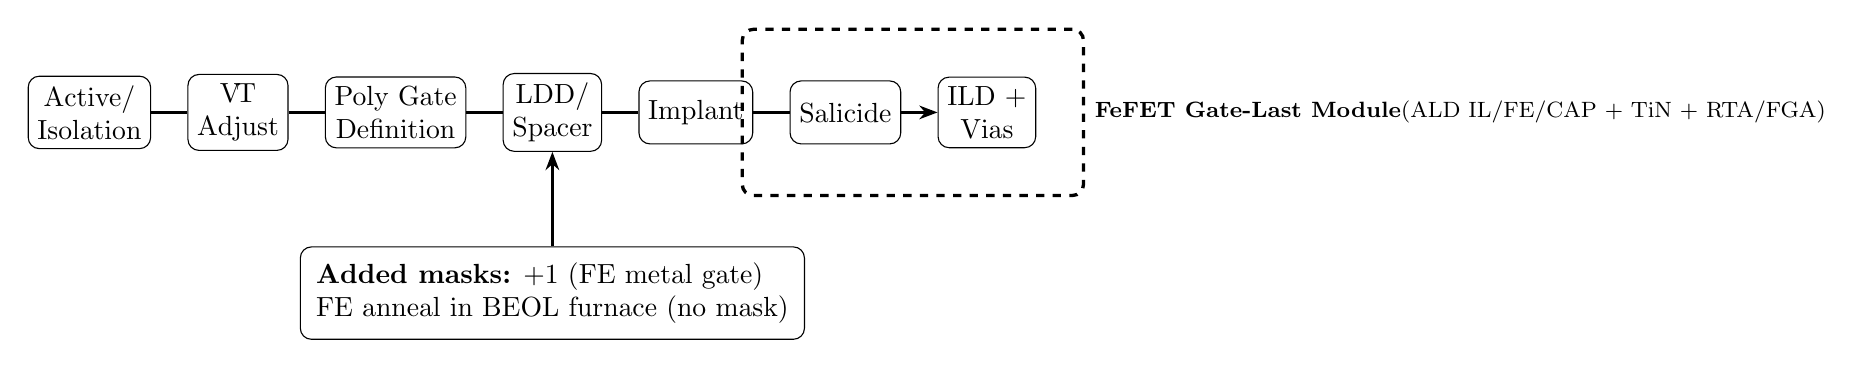
\begin{tikzpicture}[
  node distance=4.6mm,
  stage/.style={draw,rounded corners,minimum width=11mm,minimum height=8mm,align=center},
  arr/.style={-{Stealth},thick},
  ann/.style={font=\footnotesize}
]
\node[stage] (act)  {Active/\\Isolation};
\node[stage,right=of act] (vt)  {V\!T\\Adjust};
\node[stage,right=of vt]  (poly) {Poly Gate\\Definition};
\node[stage,right=of poly] (ldd)  {LDD/\\Spacer};
\node[stage,right=of ldd]  (imp)  {Implant};
\node[stage,right=of imp]  (sal)  {Salicide};
\node[stage,right=of sal]  (ild)  {ILD +\\Vias};
\draw[arr] (act) -- (vt) -- (poly) -- (ldd) -- (imp) -- (sal) -- (ild);
\node[draw,dashed,very thick,rounded corners,fit=(sal) (ild),
      inner sep=6mm,label={[ann]right:{\textbf{FeFET Gate-Last Module}\\(ALD IL/FE/CAP + TiN + RTA/FGA)}}] {};
\node[draw,rounded corners,below=12mm of ldd,align=left,inner sep=2mm] (note) {%
\textbf{Added masks:} +1 (FE metal gate)\\
FE anneal in BEOL furnace (no mask)};
\draw[arr] (note.north) to[out=90,in=-90] (ldd.south);
\end{tikzpicture}
\caption{Placement of the FeFET module within the 0.18\,$\mu$m CMOS baseline flow.}
\label{fig:flow}
\end{figure}

\maybeinput{build/process_integration_en.tex}

\section*{プロセス統合}
\maybeinput{build/process_integration_ja.tex}

\section{Experimental Conditions}
\maybeinput{build/experimental_conditions_en.tex}

\section*{実験条件}
\maybeinput{build/experimental_conditions_ja.tex}

\section{Reliability}
% --- Endurance Figure with PGFPlots ---
\begin{figure}[t]
\centering
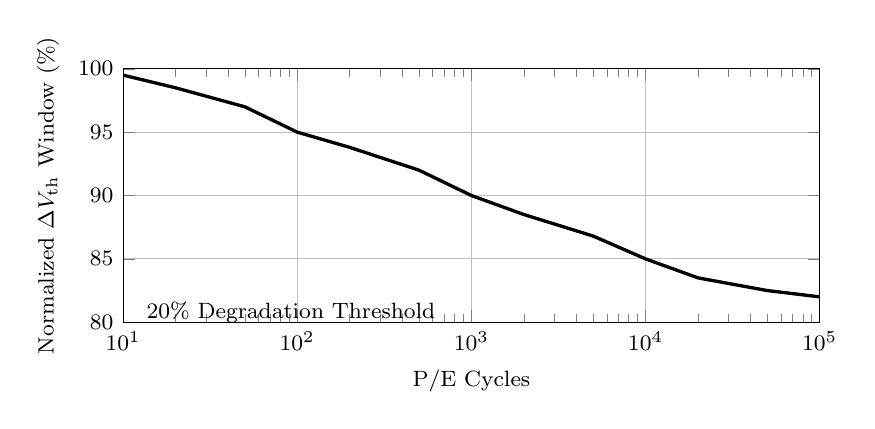
\begin{tikzpicture}
\begin{semilogxaxis}[
  width=0.86\linewidth,
  height=48mm,
  xmin=10, xmax=1e5,
  ymin=80, ymax=100,
  xlabel={P/E Cycles},
  ylabel={Normalized $\Delta V_{\mathrm{th}}$ Window (\%)},
  ymajorgrids, xmajorgrids,
  label style={font=\footnotesize},
  tick label style={font=\footnotesize},
]
\addplot[densely dashed] coordinates {(10,80) (1e5,80)};
\node[anchor=west,font=\footnotesize] at (axis cs:12,80.8) {20\% Degradation Threshold};
\addplot[very thick] table[row sep=\\]{
x   y\\
10  99.5\\
20  98.5\\
50  97.0\\
100 95.0\\
200 93.8\\
500 92.0\\
1000 90.0\\
2000 88.5\\
5000 86.8\\
10000 85.0\\
20000 83.5\\
50000 82.5\\
100000 82.0\\
};
\end{semilogxaxis}
\end{tikzpicture}
\caption{Endurance measured at $V_{\mathrm{PGM}}=X$\,V with pulse width $t=Y$\,$\mu$s (example trend).}
\label{fig:endurance}
\end{figure}

\maybeinput{build/reliability_en.tex}

\section*{信頼性}
\maybeinput{build/reliability_ja.tex}

\section{Conclusion}
\maybeinput{build/conclusion_en.tex}

\section*{結論}
\maybeinput{build/conclusion_ja.tex}

% ================= References =================
\bibliographystyle{IEEEtran}
\bibliography{refs}

% ================= Biography =================
\section*{Author Biography}
Shinichi Samizo received the M.S. degree in Electrical and Electronic Engineering from Shinshu University, Japan.  
He joined Seiko Epson Corporation in 1997, where he engaged in semiconductor device process development including 0.25--0.18\,$\mu$m CMOS, HV-CMOS, \textbf{DRAM}, FeRAM, and FinFET/GAA research.  
He also contributed to inkjet MEMS process development and thin-film piezo actuator design, leading to the productization of PrecisionCore printheads.  
His expertise covers semiconductor devices (logic, memory \textbf{[DRAM/FeRAM/SRAM]}, high-voltage mixed integration), inkjet actuators, and AI-based control education.

\section*{著者略歴}
三溝真一(Shinichi Samizo) 信州大学大学院 電気電子工学専攻 修了。  
1997年よりセイコーエプソン株式会社にて、半導体デバイスプロセス開発(0.25~0.18\,$\mu$m CMOS、HV-CMOS、\textbf{DRAM}、FeRAM、FinFET/GAA研究)に従事。  
また、インクジェットMEMSプロセス開発および薄膜ピエゾアクチュエータ設計、PrecisionCoreプリントヘッドの量産化にも携わった。  
専門分野は半導体デバイス(ロジック・メモリ〔\textbf{DRAM/FeRAM/SRAM}〕・高耐圧混載)、インクジェットアクチュエータ、AI制御・教育教材開発。

\end{document}
